\documentclass[12pt]{article}
\usepackage[paperwidth=595.92bp,paperheight=842.88bp,top=18mm,bottom=20mm,left=16mm,right=16mm,headheight=7bp,headsep=27.3bp,footskip=41.6bp]{geometry}
\usepackage{fontspec}
\usepackage{xcolor}
\usepackage{graphicx}
\usepackage{titlesec}
\usepackage{enumitem}
\usepackage{caption}
\usepackage{lastpage}
\usepackage{natbib}
\setmainfont{TeX Gyre Heros}
\newfontfamily\headfont{TeX Gyre Termes}
\definecolor{ink}{HTML}{1F1E1D}
\definecolor{muted}{HTML}{6B6B6B}
\color{ink}
\setcounter{secnumdepth}{0}
\renewcommand{\normalsize}{\fontsize{12bp}{18bp}\selectfont}
\normalsize
\setlength{\parindent}{0pt}
\setlength{\parskip}{7.5bp}
\raggedright
\hyphenpenalty=10000 \exhyphenpenalty=10000
\titleformat{\section}{\headfont\fontsize{16.5bp}{21.45bp}\selectfont}{}{0pt}{}
\titlespacing*{\section}{0pt}{26bp}{9bp}
\setlist[itemize]{leftmargin=17.5bp,itemsep=3bp,parsep=0pt,topsep=0pt,partopsep=0pt}
\captionsetup{font={small,color=muted},labelfont={color=muted},justification=raggedright,singlelinecheck=false,skip=3bp}
\renewcommand{\small}{\fontsize{10.5bp}{15bp}\selectfont}
\setlength{\bibsep}{3bp}
\bibliographystyle{plainnat}
\newcommand{\HeadLabel}{Final Report — Group 6}
\newlength{\hdrY}\setlength{\hdrY}{1pt}
\usepackage{fancyhdr}
\pagestyle{fancy}\fancyhf{}
\renewcommand{\headrulewidth}{0pt}
\fancyhead[L]{\fontsize{6bp}{7bp}\selectfont\color{muted}\HeadLabel}
\fancyfoot[R]{\fontsize{6bp}{7bp}\selectfont\color{muted}Page \thepage{} of \pageref{LastPage}}
\begin{document}
{\headfont\fontsize{24bp}{28.8bp}\selectfont Beyond Factual QA: Extending the Low-Resource Hallucination-Detector Robustness Phenomenon to Dialogue Generation and a Broader Set of Languages\par}
\vspace{18bp}\nopagebreak
{\setlength{\parskip}{6.75bp}
AI2002 – Artificial Intelligence, Fall 2026 · Track B (Research \& Development) · Group ID: 6\par
Ahmad Ali Khan (Lead, 24L-3049) · Talha Pasha (24L-3005) · Moeed Amir (24L-3060) · Bilal Kashif (24L-3036)\par}

\section{Abstract}
TBD

\section{Introduction}
TBD

\section{Related work}
TBD

\section{Data}
TBD

\section{Methodology}
TBD

\begin{figure}[h]
\centering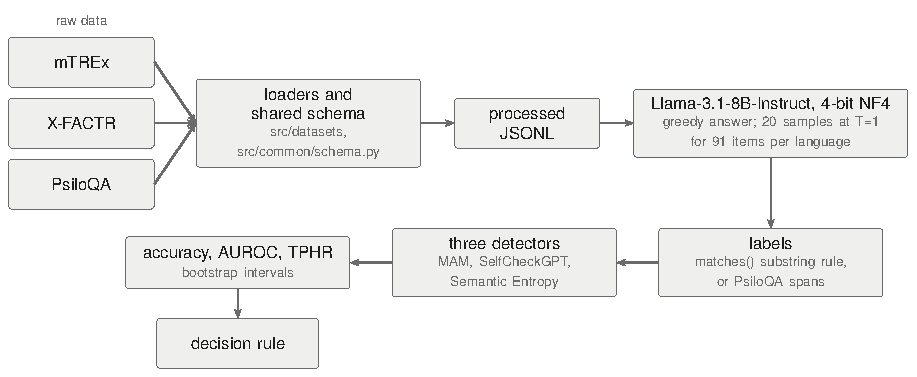
\includegraphics{figures/pipeline.pdf}
\caption{Pipeline from raw data to the decision rule.}
\end{figure}
\begin{figure}[h]
\centering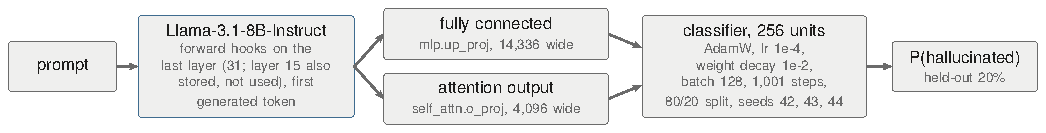
\includegraphics{figures/mam.pdf}
\caption{MAM detector.}
\end{figure}

\section{Implementation and workflow}
TBD

\section{Experimental setup}
TBD

\section{Results}
TBD

\section{Our reference run against the paper's reported results}
TBD

\section{Bias check}
TBD

\section{Error analysis}
TBD

\section{Insights}
TBD

\section{Challenges faced during implementation}
TBD

\section{Limitations}
TBD

\section{How to run and reproduce}
TBD

\section{Conclusion}
TBD

\nocite{*}
{\titleformat{\section}{\headfont\fontsize{16.5bp}{21.45bp}\selectfont}{}{0pt}{}
\section{References}
{\fontsize{10.5bp}{15bp}\selectfont\bibliography{refs}}}
\end{document}
